\chapter{Imbalanced Classification}
\label{chapter:imb-classif}


\section{Oversampling Methods}
\label{section:oversampling-methods}

Oversampling methods constitute one possible approach to solving the imbalanced classification
problem. The main goal of oversampling methods is to modify the empirical distribution by
increasing the number of samples belonging to the minority class. The empirical distribution is
modified either by duplicating the existing samples or generating new artificial samples until the
desired imbalance ratio is reached. The following text presents oversampling methods used in the
further chapters.


\subsection{Random Oversampling}
\label{subsection:random-oversampling}

The most straightforward approach to tackling the underrepresentation of a class is by duplicating
the available data samples belonging to that class. Samples to duplicate are chosen randomly with a
replacement. Bare duplication of samples may introduce completely overlapping samples, as shown in
the left scatter plot in Figure~\ref{figure:random-oversampling}. Random oversampling introduced
sixty new minority samples to balance the classes; however, we can only see twenty, as most of them
are entirely overlapping. A modification known as \textit{Random Oversampling Examples} (ROSE) was
proposed in 2012 to avoid this~\cite{rose}. It starts by randomly choosing a sample from the
minority class and then generates a new artificial sample in the close neighbourhood of the
original sample. Generating new samples close to the already existing ones enlarges the regions
occupied by the minority class~\cite{smote} and results in a better overall performance of a
classifier.

\begin{figure}
    \centering
    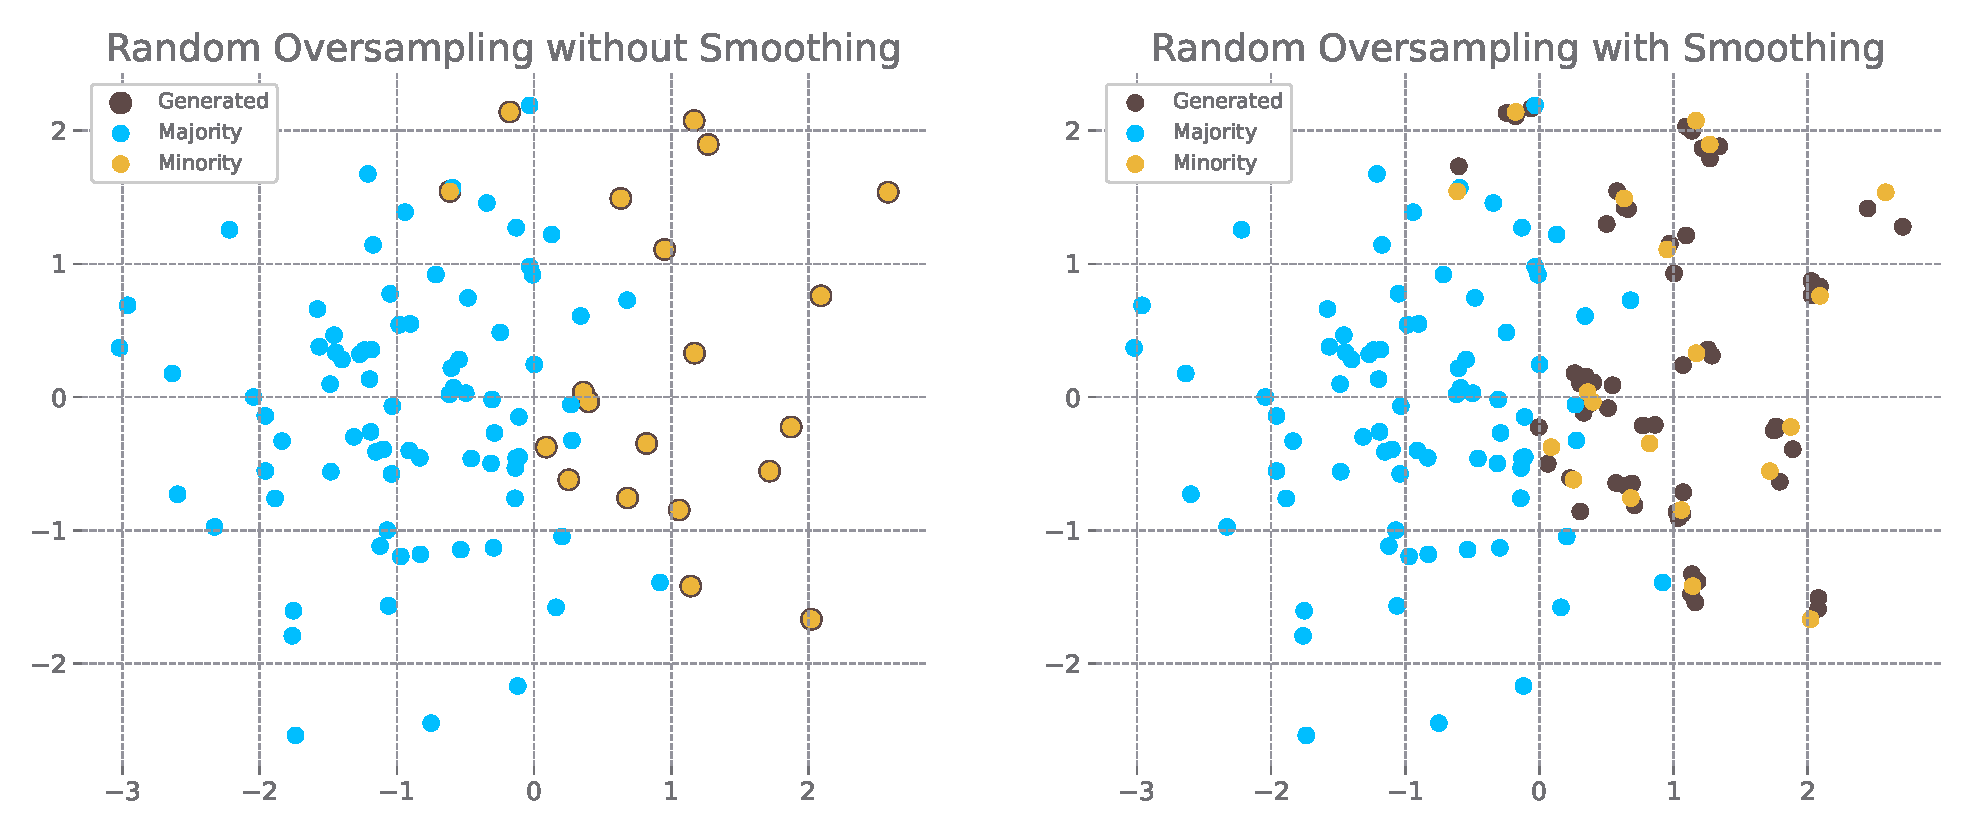
\includegraphics[width=\linewidth]{figures/random_oversampling_vs_rose.eps}
    \caption{
        \textbf{Random Oversampling vs ROSE.} The figure shows how generating new samples in the
        close neighbourhood of the original sample helps to disperse the new samples instead of
        stacking them on top of each other. In both cases, the oversampling method created sixty
        new data samples shown in a brown colour.
    }
    \label{figure:random-oversampling}
\end{figure}


\subsection{Synthetic Minority Oversampling Technique - SMOTE}
\label{subsection:smote}

SMOTE was proposed by Chawla et al.~\cite{smote} in 2002 and is one of the most widely used
imbalanced preprocessing techniques. It creates new synthetic examples on the line segments between
existing examples from the minority class. The amount of oversampling supplied by the user
determines if all minority samples participate in the oversampling. If we plan to oversample the
minority class by at least 100\%, then every existing minority sample is used; otherwise, a random
subset $\mathcal{S} \subseteq {S_{min}}$ of samples is chosen. The algorithm looks at k-nearest
neighbours, where $k$ is again a hyperparameter supplied by the user, of an existing minority
example $\mathbf{x}_i$ and randomly chooses a subset of the neighbours $\mathcal{N} =
\{\,\mathbf{x} \mid \mathbf{x} \in \mathrm{kNN}(\mathbf{x}_i)\,\}$. The subset's size also depends
on the amount of oversampling we plan to do. If, for example, we plan to oversample the minority
class by 200\%, then for each existing minority sample, the subset will contain two randomly chosen
neighbours. If, on the other hand, the amount of oversampling is less than 100\%, the algorithm
generates one new artificial sample for each existing sample in the subset $\mathcal{S}$. For each
neighbour $\mathbf{x}_j \in \mathcal{N}$, the algorithm computes the difference between
$\mathbf{x}_i$ and $\mathbf{x}_j$, multiplies it by a random number $r$ chosen uniformly from the
interval $(0, 1)$, and finally adds it to the original sample $\mathbf{x}_i$. The final formula for
generating a new artificial sample is:
\begin{equation}
    \mathbf{x}_{new} = \mathbf{x}_i + r \cdot (\mathbf{x}_i - \mathbf{x}_j)
    \label{equation:smote}
\end{equation}


\subsection{Borderline SMOTE}
\label{subsection:bordeline-smote}

One drawback the SMOTE algorithm has is that it considers all minority samples to be of the same
importance. Minority samples surrounded largely by majority samples are far more prone to
misclassification than those surrounded predominantly by minority samples. Borderline
SMOTE~\cite{borderline-smote} tries to select only endangered minority samples and performs the
original SMOTE algorithm only on those samples, as shown in
Figure~\ref{figure:smote-vs-borderline}. The algorithm first finds k-nearest neighbours for each
$\mathbf{x}_i \in S_{min}$. Next, it selects only those minority samples with at least half of
their neighbours belonging to the majority class. One interesting case is when all of the
neighbours of a minority sample belong to the majority class. In this case, the minority sample is
considered noise in the data and is not selected. These conditions can be summarised as follow:
\begin{equation}
    \mathcal{S} = \{\mathbf{x} \mid \mathbf{x} \in S_{min} \land \frac{k}{2} \leq \, \mid
        \mathrm{kNN}(\mathbf{x}_i) \cap S_{maj} \mid \, < k\}.
\end{equation}
The resulting set $\mathcal{S}$ is sent to the SMOTE algorithm to generate new artificial samples
on the border.

\begin{figure}
    \centering
    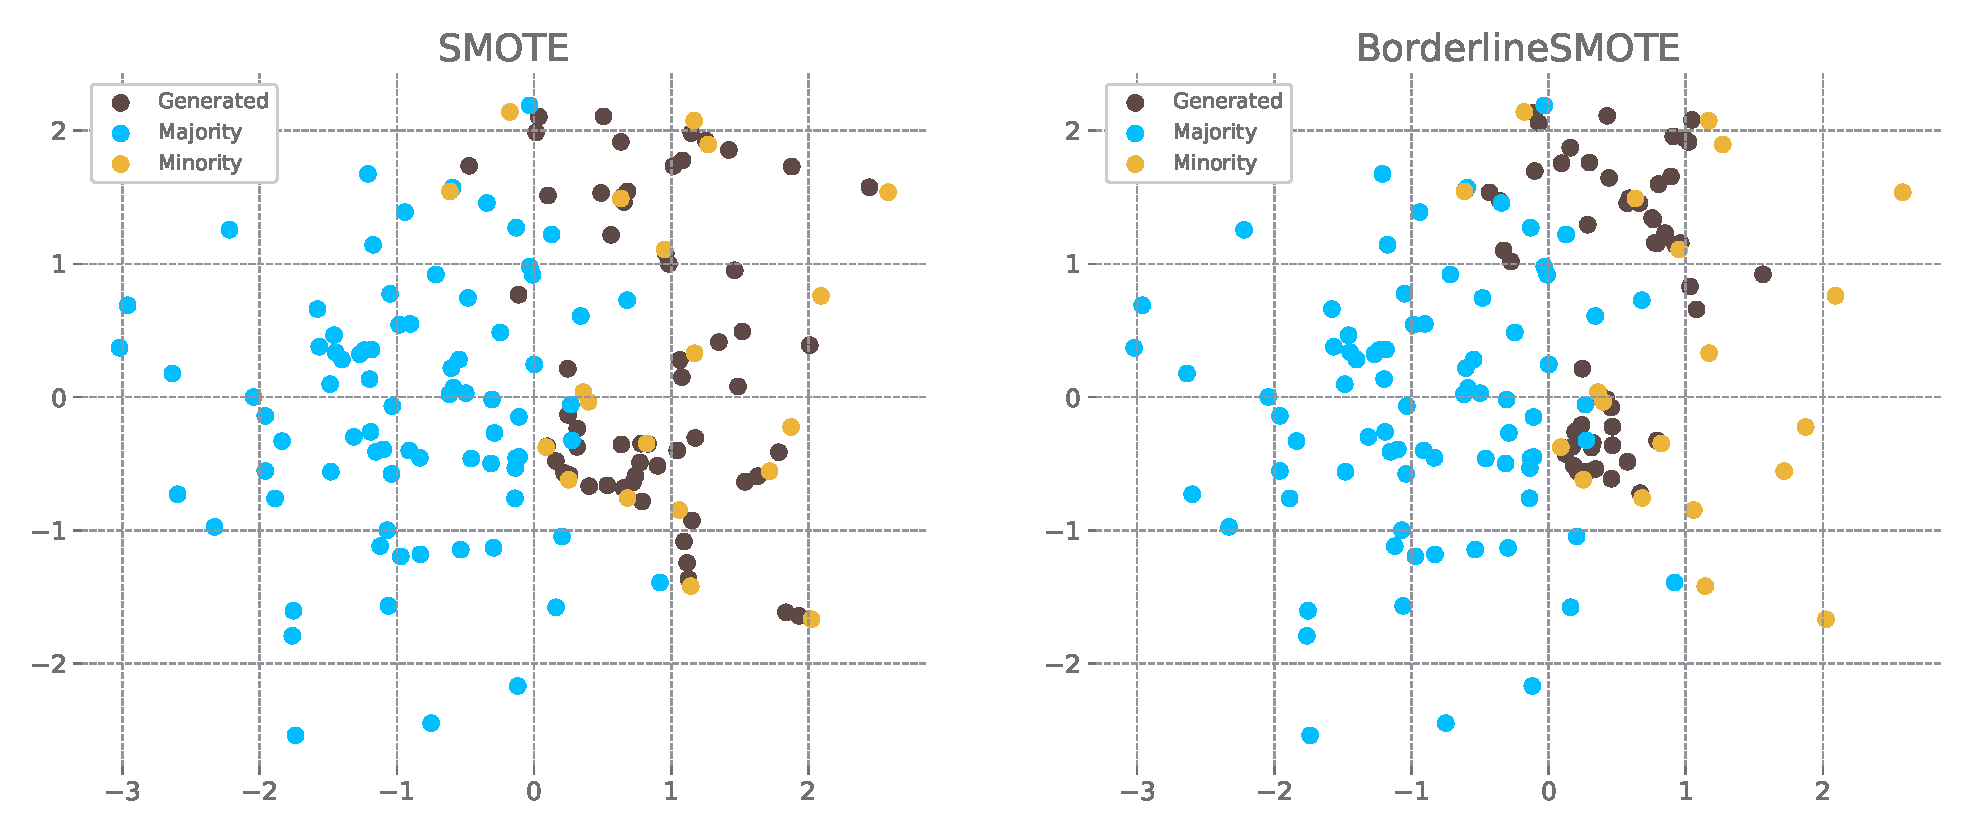
\includegraphics[width=\linewidth]{figures/smote_vs_borderlinesmote.eps}
    \caption{
        \textbf{SMOTE vs Borderline SMOTE.} The figure shows how the Borderline SMOTE algorithm,
        depicted on the right, focuses its attention on endangered minority samples near the
        decision boundary, while SMOTE sees every minority sample having the same importance. The
        most noticeable difference can be seen on the far right side of the figures. SMOTE
        generates new samples in those regions, whereas Borderline SMOTE does not, as those samples
        are far from the decision boundary.
    }
    \label{figure:smote-vs-borderline}
\end{figure}


\subsection{SVM SMOTE}
\label{subsection:svm-smote}

SVM~SMOTE~\cite{svm-smote} also enhances the SMOTE algorithm by focusing on endangered minority
samples. It starts by training a support vector machine classifier~\ref{section:svm} using the
original dataset. The SVM classifier identifies the so-called support vectors in the original data.
These are the training samples that approximate the optimal decision boundary. SVM SMOTE uses these
samples to generate artificial samples near the approximated optimal decision boundary using
interpolation (SMOTE) or extrapolation depending on the density of the majority class around it.
The number of artificial samples to generate is distributed evenly among minority class support
vectors. For each minority support vector $\mathbf{x}_i$, find k-nearest neighbours on the whole
training data set. If minority samples account for less than half of the neighbours, create a new
artificial sample by interpolating between $\mathbf{x}_i$ and its neighbour $\mathbf{x}_j \in
\mathrm{kNN}(\mathbf{x}_i)$ to strengthen the presence of the minority class in crowded regions.
If, on the other hand, there are more minority samples among the neighbours than majority samples,
the algorithm performs extrapolation to enlarge the area occupied by the minority class.

\begin{figure}
    \centering
    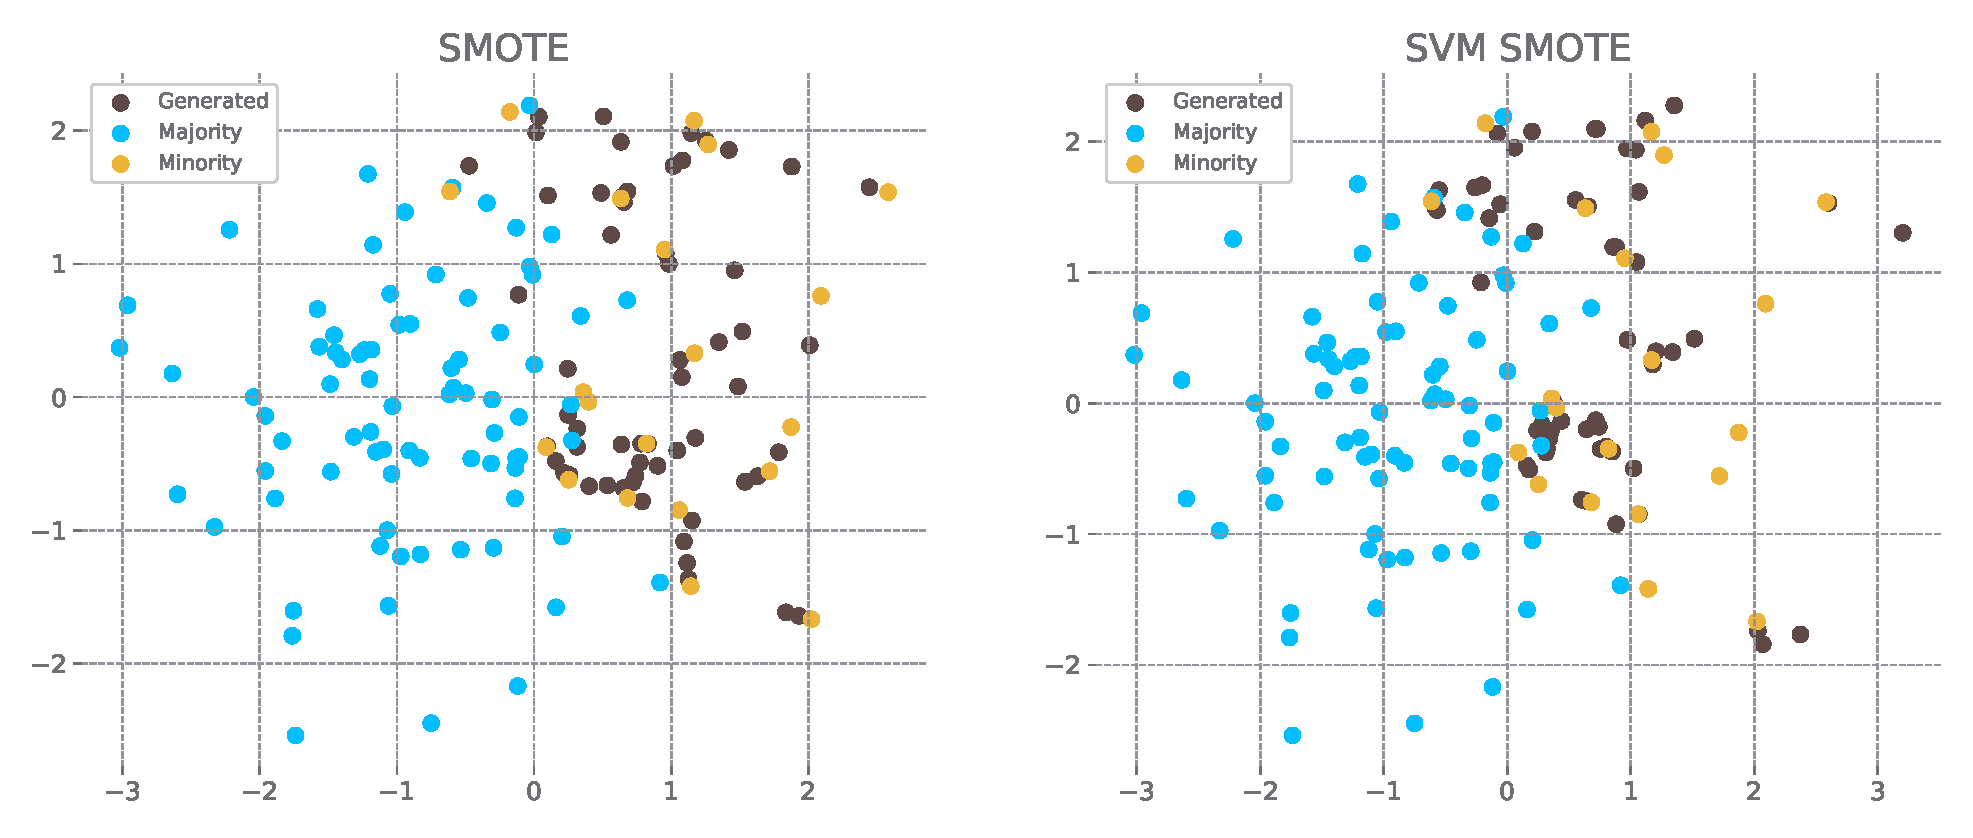
\includegraphics[width=\linewidth]{figures/smote_vs_svmsmote.eps}
    \caption{
        \textbf{SMOTE vs SVM SMOTE.} The figure shows how SVM SMOTE, shown on the right, prefers
        generating samples, shown in a brownish colour, near the decision boundary to strengthen
        the presence of samples from the minority class. In contrast, the original implementation
        of the SMOTE algorithm generates new samples near every original sample from the minority
        class regardless of its position. Furthermore, we can see the interpolation in the dense
        regions in the centre of the plot around the point $(0, 0)$ and the extrapolation on the
        far right.
    }
    \label{figure:smote-vs-svmsmote}
\end{figure}


\subsection{KMeans SMOTE}
\label{subsection:kmeans-smote}

Employing a uniform probability to choose minority samples to oversample is another drawback of
SMOTE. It increases the likelihood of further inflating regions with many minority samples and
neglecting sparse regions~\cite{kmeans-smote}. KMeans~SMOTE~\cite{kmeans-smote} is an enhancement
of SMOTE that focuses on this issue. In the first phase, it employs the KMeans clustering
algorithm~\ref{section:kmeans} to cluster data samples into $k$ groups based on the euclidean
distance. Clustering helps focus the attention on the regions where minority samples are dominant,
preventing SMOTE from generating unnecessary noise by interpolating noisy minority
samples~\cite{kmeans-smote}. Once the clusters were identified, KMeans SMOTE retains only those
clusters that contain more minority samples than majority samples, i.e. clusters whose imbalance
ratio is greater than 1. Next, it computes how many artificial examples must be generated in each
selected cluster based on its density of minority samples. This enables the subsequent step to
generate more samples in sparse regions, thus achieving balanced between-class and
\emph{within-class} distribution. The balanced within-class distribution ensures approximately the
same density of minority samples in the minority class regions. The cluster's density is computed,
for each cluster $f$, as follows:

\begin{enumerate}
    \item Calculate a distance matrix between minority samples belonging to cluster $f$
    \item Calculate a mean distance $\mathrm{mean\_distance(f)}$
    \item Calculate the cluster's density as $\mathrm{density(f)} = \frac{\mid S_{min}
        \mid}{\mathrm{mean\_distance(f)}^m}$, where $m$ is the dimension of a sample
    \item Calculate $\mathrm{sparsity(f)} = \frac{1}{\mathrm{density(f)}}$
\end{enumerate}

Finally, normalise $\mathrm{sparsity(f)}$ to be a distribution. Normalisation allows us to multiply
each cluster's sparsity by the total number of data to generate to obtain the portion of samples to
generate in each cluster. The last step of the algorithm consists of performing the SMOTE algorithm
in each cluster separately to generate the needed number of samples to reach the specified ratio of
majority and minority samples.

\begin{figure}
    \centering
    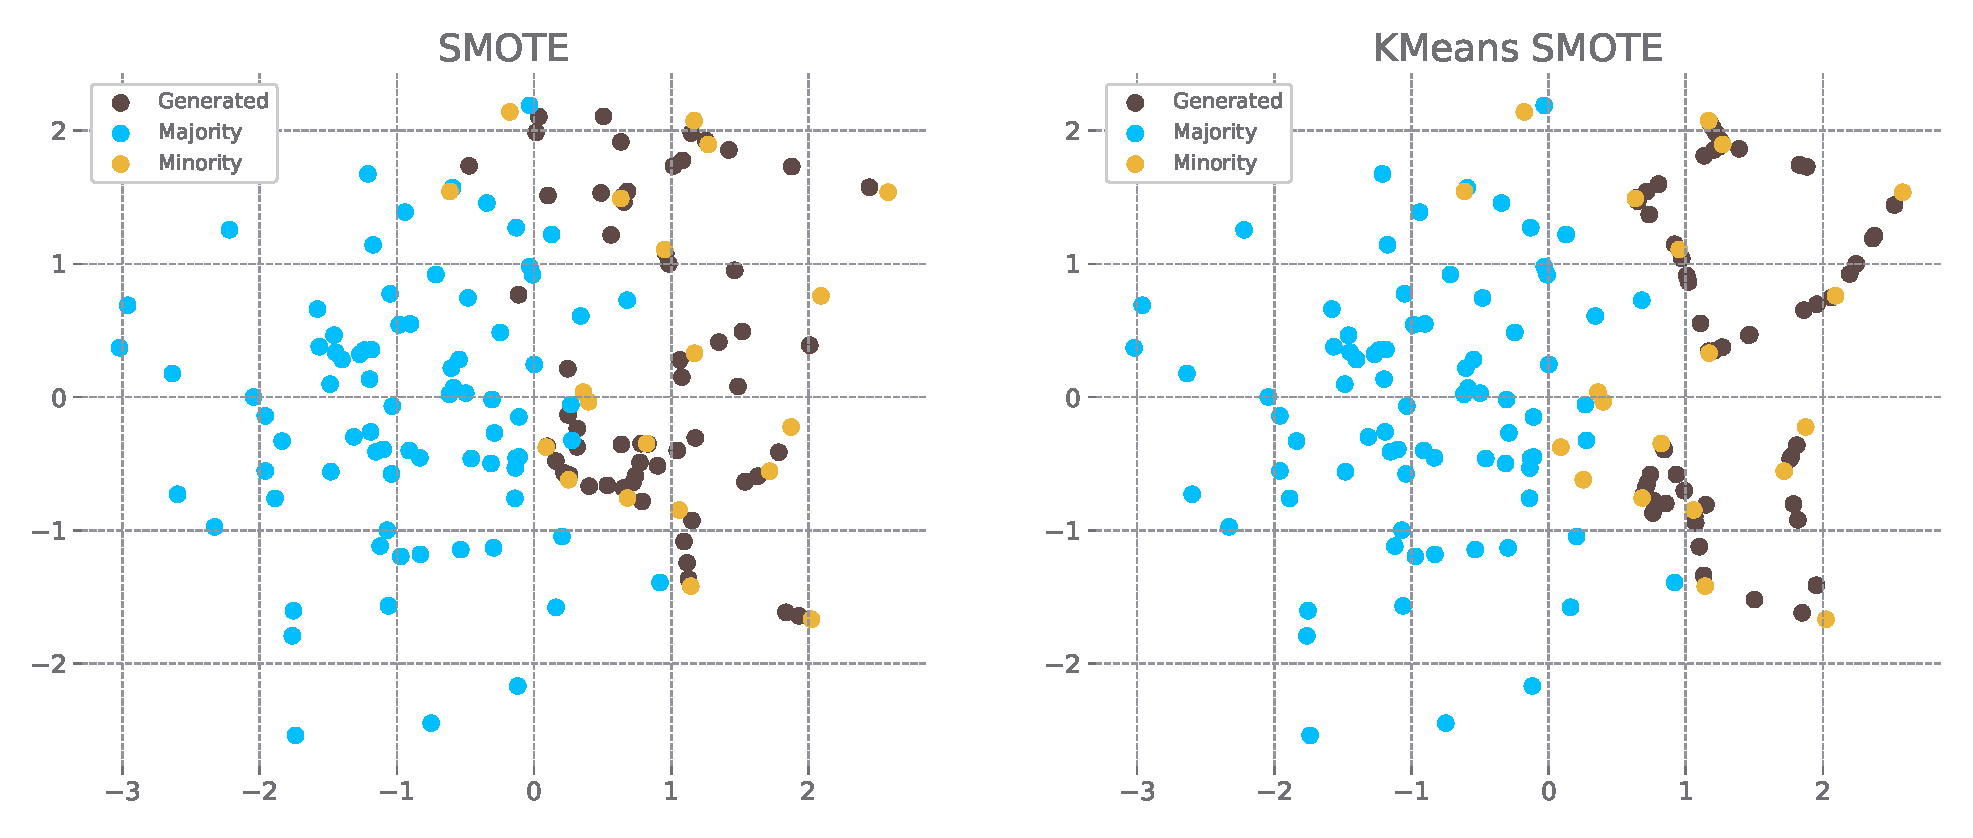
\includegraphics[width=\linewidth]{figures/smote_vs_kmeanssmote.eps}
    \caption{
        \textbf{SMOTE vs KMeans SMOTE.} The figure compares SMOTE and KMeans SMOTE. We can see how
        SMOTE generates many new samples, shown in brown, slightly below the point $(0, 0)$. KMeans
        SMOTE, on the other hand, does not generate almost any new samples in that region as
        samples in that region can be considered noise. The same reasoning can be applied to
        samples at the top, surrounded predominantly by the majority class samples.
    }
    \label{figure:smote-vs-kmeanssmote}
\end{figure}
